\section{фи 29 DNA polymerase}

\subsection{Нормальное название}

Специфический субдомен ДНК-полимеразы Ф29(фермент вируса Ф29) обеспечивает процессивность и способность замещения цепи.

\subsection{Абстракт}

Недавние кристаллографические  исследования ДНК-полимеразы Ф29 обеспечили понимание процессивности и замещения цепи. (Здесь, процессивность ДНК полимеразы -- среднее число нукелеотидов, присоединяемых ферментом за один акт связывания.)
Специфическая вставка TPR2(названная так по концевой области белка)  вместе с доменами, образует два тора, способных связываться с ДНК. Для анализа функциональной роли TPR2  была сконструирована мутантная версия с делецией аминокислот от 398 до 420. В результате биохимического анализа было выявлено, что снижается ДНК-связывающая способность, следовательно процессивность. Также удаление участка TPR2 лишает ДНК-полимеразу возможности выполнять замещение цепи, необходимое для синтеза ДНК.

\subsection{Картинки}

\begin{figure}[H]
	\centering
	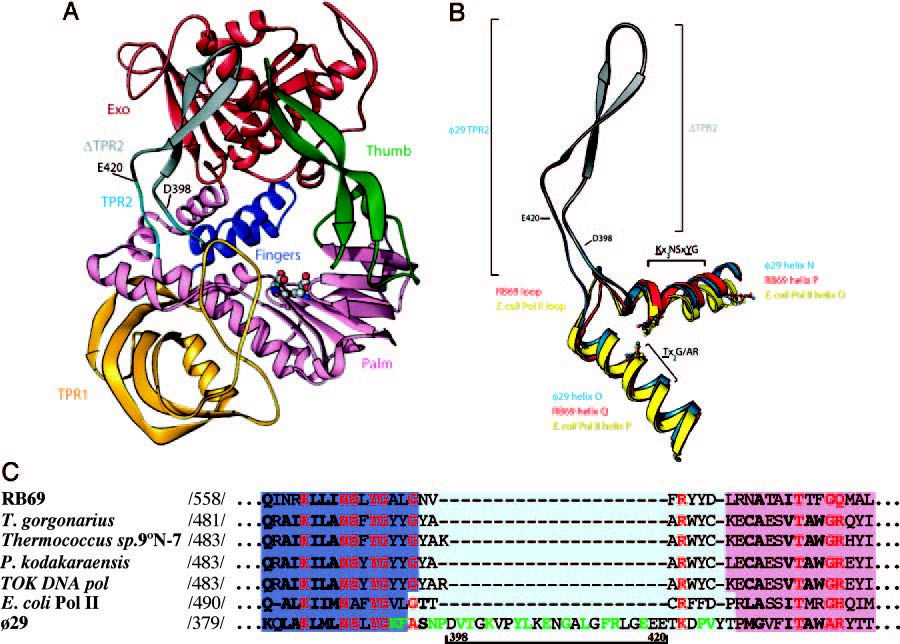
\includegraphics[width=0.5\linewidth]{1_1}
	\caption{1А: структура днк полимеразы, показана локализация вставки TPR2; 1B: выравнивание структур мутантного варианта и дикого типа; 1С: выравнивание последовательностей нескольких бактерий и мутантной версии с делецией, выделены консервативные мотивы.}
	\label{fig:1_1}
\end{figure}

\begin{figure}[H]
	\centering
	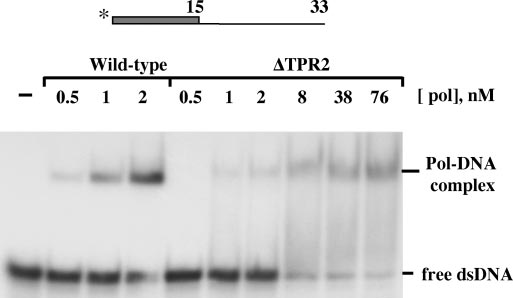
\includegraphics[width=0.5\linewidth]{1_2}
	\caption{Электрофорез, показывающий высокую процессивность/возможность замещения цепи. Здесь надо обратить внимание на оси, в зависимости от концентрации pol/dNTP показано преимущество дикого типа перед мутантным вариантом с делецией.}
	\label{fig:1_2}
\end{figure}

\begin{figure}[H]
	\centering
	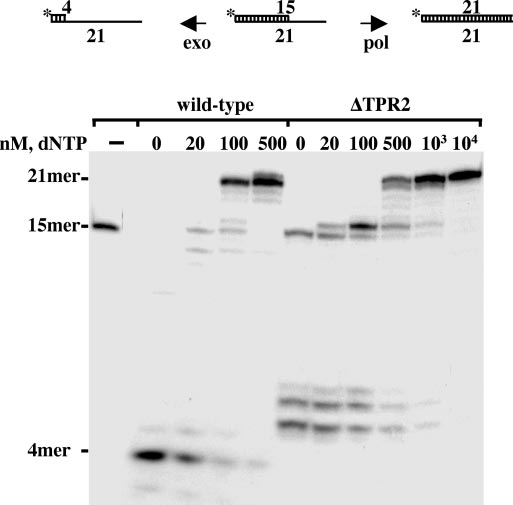
\includegraphics[width=0.5\linewidth]{1_3}
	\caption{Электрофорез, показывающий высокую процессивность/возможность замещения цепи. Здесь надо обратить внимание на оси, в зависимости от концентрации pol/dNTP показано преимущество дикого типа перед мутантным вариантом с делецией.}
	\label{fig:1_3}
\end{figure}

\begin{figure}[H]
	\centering
	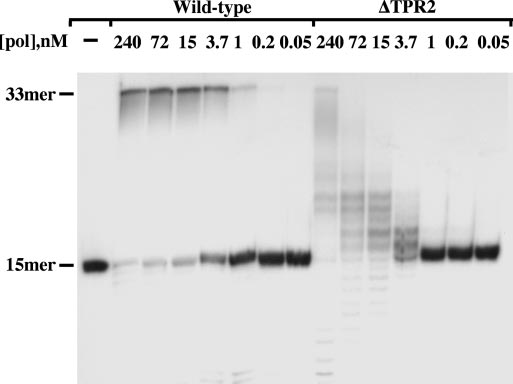
\includegraphics[width=0.5\linewidth]{1_4}
	\caption{Электрофорез, показывающий высокую процессивность/возможность замещения цепи. Здесь надо обратить внимание на оси, в зависимости от концентрации pol/dNTP показано преимущество дикого типа перед мутантным вариантом с делецией.}
	\label{fig:1_4}
\end{figure}

\begin{figure}[H]
	\centering
	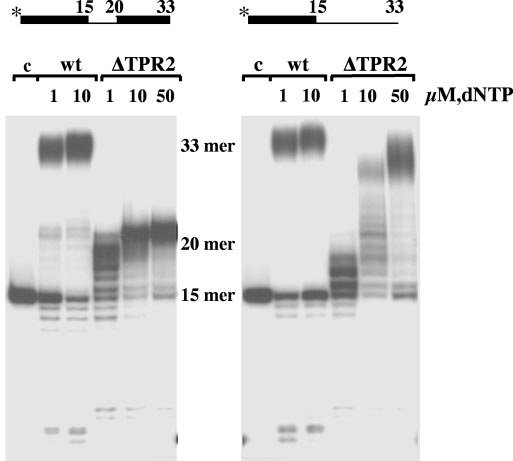
\includegraphics[width=0.5\linewidth]{1_5}
	\caption{Электрофорез, показывающий высокую процессивность/возможность замещения цепи. Здесь надо обратить внимание на оси, в зависимости от концентрации pol/dNTP показано преимущество дикого типа перед мутантным вариантом с делецией.}
	\label{fig:1_5}
\end{figure}

\begin{figure}[H]
	\centering
	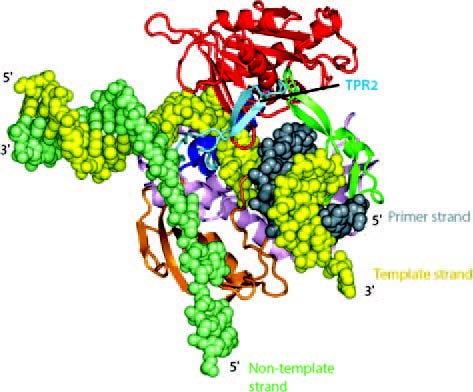
\includegraphics[width=0.5\linewidth]{1_6}
	\caption{Моделирование высокой процессивности и замещения цепи.}
	\label{fig:1_6}
\end{figure}